\begin{graphicspathcontext}{{./chapters/hmas/imgs/},{./chapters/hmas/imgs/auto/},\old}

\sidecite{Rodriguez2026}
\begin{frame}{SARL: a Brief Reminder}
	\begin{block}{SARL is an agent-oriented programming language}
		\begin{itemize}
		\item Designed for programming agent-based and holonic systems
		\item Built-in \Emph{event-driven} communication model
		\item Core concepts: \code{agent}, \code{capacity}, \code{skill}, \code{behavior}, \code{event}
		\item Each agent lives in an \code{AgentContext} (an event space + agent registry)
		\item An agent can create an \Emph{inner context} --- this is the holonic mechanism
		\end{itemize}
	\end{block}
	\begin{exampleblock}{Built-in capacities for holonic systems}
		\begin{description}
		\item[InnerContextAccess] Access the inner context and its members
		\item[Lifecycle] Spawn agents in any context (\code{spawnInContext})
		\item[DefaultContextInteractions] Interact in the outer context
		\end{description}
	\end{exampleblock}
\end{frame}

\begin{frame}[t]{SARL Holonic Architecture}
	\smaller
	\begin{center}
		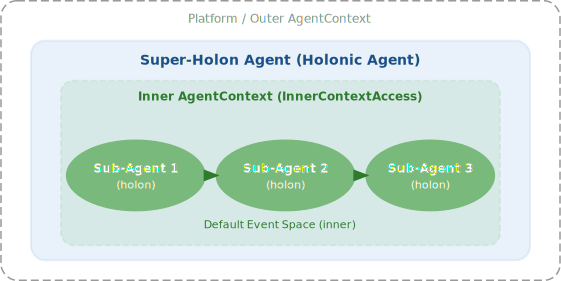
\includegraphics[width=.6\linewidth]{hmas_sarl_inner_context}
	\end{center}
	\begin{block}{How it works}
		\begin{itemize}
		\item An agent possesses an \emph{inner context} (via \code{InnerContextAccess})
		\item Sub-agents are spawned \emph{inside} this inner context using \code{spawnInContext}
		\item The super-holon broadcasts events to all members via the inner context's default space
		\item Sub-agents emit events upward by targeting the super-holon's address in the outer context
		\end{itemize}
	\end{block}
\end{frame}

\begin{frame}[fragile]{Example: Defining Events for a Holonic System}
	\begin{sarllisting}
// Event sent by the super-holon to sub-holons
event TaskAssigned {
	val taskId : int
	val description : String
}

// Event sent by a sub-holon to report its result
event TaskResult {
	val taskId : int
	val result : String
}
	\end{sarllisting}
\end{frame}

\begin{frame}[t,fragile]{Example: The Sub-Holon (Worker Agent)}
	\begin{sarllisting}[basicstyle=\scriptsize]
agent WorkerHolon {
	uses Logging, DefaultContextInteractions, Lifecycle

	// React to a task assigned by the super-holon
	on TaskAssigned {
		info("Worker received task #" + occurrence.taskId)
		// ... do work ...
		val res = "Result of task " + occurrence.taskId
		// Send result back to the outer space
		emit(new TaskResult(occurrence.taskId, res))
	}

	on Destroy {
		info("Worker is shutting down")
	}
}
	\end{sarllisting}
	\vspace{-.5cm}
	\begin{compactitemize}
	\item Workers receive \code{TaskAssigned} from the inner event space
	\item They emit \code{TaskResult} back into the same space
	\end{compactitemize}
\end{frame}

\begin{frame}[t,fragile]{Example: The Super-Holon (Holonic Agent)}
	\begin{sarllisting}[basicstyle=\scriptsize]
agent SuperHolon {
	uses Logging, Lifecycle, InnerContextAccess
	uses DefaultContextInteractions

	val NUM_WORKERS = 3
	var resultsReceived = 0

	// When the super-holon starts, spawn worker sub-holons
	on Initialize {
		info("SuperHolon starting, spawning workers...")
		val innerCtx = getInnerContext
		for (i : 1..NUM_WORKERS) {
			// Workers live INSIDE the inner context
			spawnInContext(WorkerHolon, innerCtx)
		}
	}
//[...]
	\end{sarllisting}
	\vspace{-.5cm}
	\begin{compactitemize}
	\item \code{getInnerContext()} returns the super-holon's own inner MAS
	\item \code{spawnInContext(WorkerHolon, innerCtx)} creates a sub-holon inside it
	\end{compactitemize}
\end{frame}

\begin{frame}[fragile]{Example: The Super-Holon (Holonic Agent) \insertcontinuationtext}
	\begin{sarllisting}[basicstyle=\scriptsize]
	// React to an external task request (from outer context)
	on TaskAssigned [isInnerDefaultSpace(occurrence.source)] == false] {
		info("SuperHolon received task, delegating to workers...")
		// Forward the task to ALL workers via the inner event space
		val innerSpace = getInnerDefaultSpace
		innerSpace.emit(
			getInnerDefaultSpace.getAddress(getID),
			new TaskAssigned(occurrence.taskId, occurrence.description))
	}
	// Collect results from workers
	on TaskResult [isInInnerDefaultSpace(occurrence)] {
		resultsReceived++
		info("Got result: " + occurrence.result)
		if (resultsReceived >= NUM_WORKERS) {
			// Aggregate and emit a global result to the outer context
			emit(new TaskResult(-1, "All subtasks completed."))
		}
	}
}
	\end{sarllisting}
\end{frame}

\begin{frame}[t,fragile]{Example: A Three-Level Holarchy in SARL}
	\begin{sarllisting}[basicstyle=\scriptsize]
agent RootHolon {
	uses Logging, Lifecycle, InnerContextAccess

	on Initialize {
		info("RootHolon: creating two super-holons")
		val inner = getInnerContext
		spawnInContext(SuperHolon, inner)  // Super-holon A
		spawnInContext(SuperHolon, inner)  // Super-holon B
	}

	// Observe the global state of the holarchy
	on TaskResult [isInInnerDefaultSpace(occurrence)] {
		info("Root received aggregated result: " + occurrence.result)
	}
}
	\end{sarllisting}
	\vspace{-.5cm}
	\begin{compactitemize}
	\item \code{RootHolon} is the top of a 3-level holarchy
	\item \code{SuperHolon} instances are at level 2 and each spawns \code{WorkerHolon} at level 1
	\item The structure mirrors the holarchy defined earlier
	\end{compactitemize}
\end{frame}

\begin{frame}[fragile]{Example: Dynamic Membership}
\begin{sarllisting}[basicstyle=\scriptsize]
event NewMemberRequest {
	val requesterAddress : Address
}

agent DynamicSuperHolon {
	uses Logging, Lifecycle, InnerContextAccess
	uses DefaultContextInteractions

	// Accept a new worker on request
	on NewMemberRequest {
		info("Accepting new member into inner context")
		spawnInContext(WorkerHolon, getInnerContext)
		// Optionally notify the new agent via its address
	}

	// A worker can also leave gracefully
	on AgentKilled {
		info("A member has left: " + occurrence.source)
	}
}
	\end{sarllisting}
	\vspace{-.5cm}
	\begin{compactitemize}
	\item Holonic membership is \emph{dynamic}: holons join and leave at runtime
	\item \code{AgentKilled} notifies the super-holon when a member exits
	\end{compactitemize}
\end{frame}

\begin{frame}[fragile]{Example: Capacity for Holonic Coordination}
	\begin{sarllisting}[basicstyle=\scriptsize]
// Capacity: what a super-holon must be able to do
capacity HolonicCoordination {
	def delegateTask(task : TaskAssigned)
	def collectResult(result : TaskResult)
	def getMemberCount : int
}

// Skill: how InnerContextAccess realises it
skill DefaultCoordinationSkill
		implements HolonicCoordination {
	uses InnerContextAccess

	def delegateTask(task : TaskAssigned) {
		getInnerDefaultSpace.emit(
		getInnerDefaultSpace.getAddress(owner.ID), task)
	}

	def collectResult(result : TaskResult) { /* aggregate */ }

	def getMemberCount : int { getMemberAgentCount }
}
	\end{sarllisting}
\end{frame}

\end{graphicspathcontext}

\endinput

